
\chapter{Methods}

\label{Methods} 

This chapter describes in detail the methods for whatever activities were necessary for your project – e.g., data gathering, data analysis, requirements analysis, design, implementation, testing/evaluation, etc. Your choice of methods should be discussed and justified in view of the project objectives, and with reference to the pertinent literature. Report not only what methods you applied in generic terms, but what you actually did: sufficient information about dates and details for your reader to understand how you ran your project, rather than just how one could run any similar project.  

Report in this chapter what you did, not what you produced or found as a 
result (which goes under Results).  
  
Note: only use the word ‘methodology’ if you know what it means!  

%% On RELU not actually being differentiable:
%Some of the hidden units included in this list are not actually differentiable %at
%all input points. For example, the rectified linear function g (z) = max{0, z} is not
%differentiable at z = 0. This may seem like it invalidates g for use with a gradientbased
%learning algorithm. In practice, gradient descent still performs well enough
%for these models to be used for machine learning tasks. This is in part because
%neural network training algorithms do not usually arrive at a local minimum of
%the cost function, but instead merely reduce its value significantly,
%Because we do not
%expect training to actually reach a point where the gradient is 0 , it is %acceptable
%for the minima of the cost function to correspond to points with undefined gradient.
%Hidden units that are not differentiable are usually non-differentiable at only a
%small number of points.
% pg 207 Goodfellow
% This section from same book pg 475, maybe better in Context
%Another important push, still ongoing, has been towards end-to-end deep
%learning speech recognition systems that completely remove the HMM. The first
%major breakthrough in this direction came from Graves et al. (2013) who trained
%a deep LSTM RNN (see section 10.10), using MAP inference over the %frame-tophoneme
%alignment, as in LeCun et al. (1998b) and in the CTC framework (Graves
%et al., 2006; Graves, 2012).

% Batch normalization - in the context of preprocessing data for our trainng

\cite{ioffe2015batch, 7005077}
define Internal Covariate Shift as the change in the
distribution of network activations due to the change in
network parameters during training. To improve the training, we seek to reduce the internal covariate shift. By
fixing the distribution of the layer inputs x as the training
progresses, we expect to improve the training speed. I
"It has
been long known (LeCun et al., 1998b; Wiesler \& Ney,
2011) that the network training converges faster if its inputs are whitened – i.e., linearly transformed to have zero means and unit variances, and decorrelated. "
However, since x is affected by
W, b and the parameters of all the layers below, changes
to those parameters during training will likely move many
dimensions of x into the saturated regime of the nonlinearity and slow down the convergence. This effect is
amplified as the network depth increases.
 In practice,
the saturation problem and the resulting vanishing gradients are usually addressed by using Rectified Linear Units
(Nair \& Hinton, 2010) ReLU(x) = max(x, 0), careful
initialization (Bengio \& Glorot, 2010; Saxe et al., 2013),
and small learning rates. If, however, we could ensure
that the distribution of nonlinearity inputs remains more
stable as the network trains, then the optimizer would be
less likely to get stuck in the saturated regime, and the
training would accelerate.

\cite{lecun2012efficient}
Lecun points out:
Stochastic learning is usually much faster than batch learning, results in better solutions, particularly on large redundant datasets. The idea being since there is a lot of repetition (similar frames is dataset). SGD also works well because nonlinear networks usually have multiple local minima of different depths. The noise present in the updates can results jumping into the basin of another, possibly deeper, local minimum. Networks learn the fastest from the most unexpected sample, so examples should be chosen with the maximum information content by means of shuffling the training set, however care must be taken not to apply this technique with data that contains outliers

In the case of "In Bengio et al.’s paper [6], the analysis of the problem of gradient decays
is generalized to parameterized dynamical systems (hence including second
order and other recurrent architectures)" \cite{hochreiter2001gradient}
% LC - 14 pages

\section{ROS}
The Robot Operating System (\cite{quigley2009ros}) is middleware, that is, placed between the operating system an the application program. It helps manage complexity and distributed systems, such as a managing the process of recording several sensor outputs in a moving vehicle. The term "plumbing" is sometimes used, as parts of a distributed application are connection with "data pipes".  
ROS was used to store data from the FORD AV dataset.


\section{Driving Simulators}

Two driving simulators were trialed, an earlier version of Udacity (\cite{UdacityCarSim}) and SDSandbox (\cite{SDSandboxSim}). Both use the Unity game engine. The former had a large user base on account of the accompanying MOOC (Massive Online Open Course), which has since started using the Unreal (\cite{unrealengine}) based Carla (\cite{Dosovitskiy17}) sim. SDSandbox is actively developed for the open source Donkey Car autonomous vehicle (\cite{DonkeyCar2020} and used by the do-it-yourself model-scale autonomous-vehicle community DIY Robocars (\cite{DIYRobocars2020} (\cite{DIYRobocars2020}). The majority of this community still uses behavioral learning to train their self-driving CNNs (see correspondence with main maintainer in \ref{corr:ellerbach}
).  
 
Both simulators are equivalent in the sense of acting as a data generator and also as a testing environment for self-driving CNNs. The difference being SDSandbox is able to generate data using, in addition to manual steering, a self-driving proportional–integral–derivative-like closed loop controller as implemented in PIDController.cs source code file (\cite{SDSandboxSim}). The feature makes generating training sets less laborious. The manual option being, a simulated car must be manually steered around the track a number of times. The process of gathering training data, manual or automated, creates a set of images and a set of corresponding steering angles, forming a labelled dataset.
The data is then ready to be processed and presented to a neural network.

Both legacy Udacity and SDSandbox also run in autonomous driving modes (Fig. \ref{fig:UdacitySdSandboxAutonomous}) the options being \textit{AUTONOMOUS MODE} and \textit{Auto Drive w Rec} respectively. Output image sizes are 320x160 and 160x120 respectively.


\begin{figure}[h!]
\centering
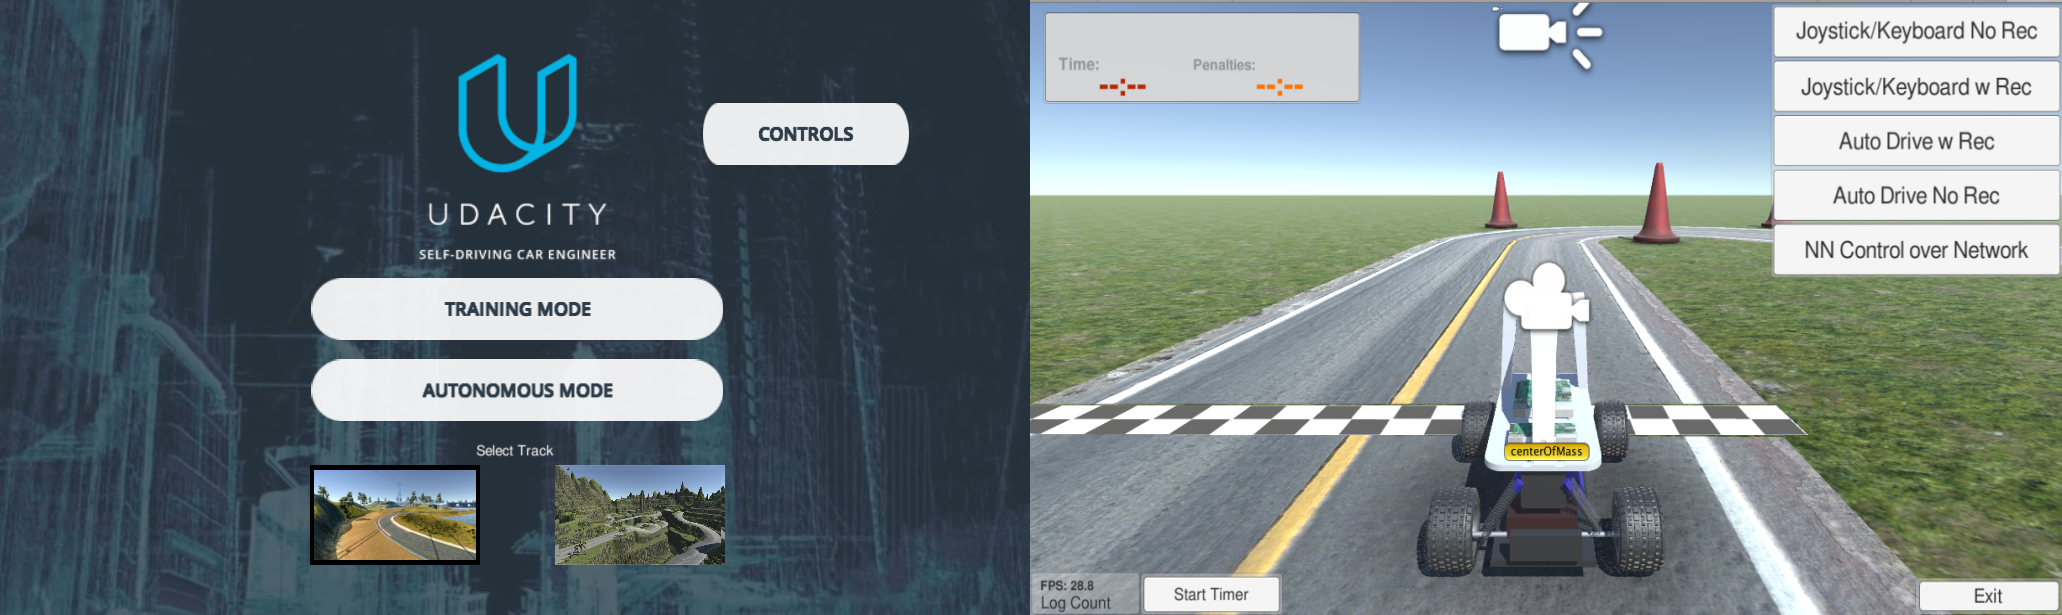
\includegraphics[width=\textwidth]{UdacitySdSandboxSim.png}
\caption{Left to right: legacy Udacity and SDSandbox Autonomous Driving Simulators}
\label{fig:UdacitySdSandboxAutonomous}
\end{figure}

Setting up the simulator and prediction engine is further detailed in Appendix
\ref{RunningCarSimulatorForInference}.

\subsection{Installing the driving simulator}
\label{recording-one-lap}
\textit{Unity Hub} is downloaded and run.

The code is cloned from:
\begin{verbatim}
git clone https://github.com/dsikar/sdsandbox    
\end{verbatim}
This will download the source code to the sdsandbox directory.

Unity Hub is then run:
\begin{verbatim}
$ sudo ./UnityAppImage --no-sandbox
\end{verbatim}

The project can then be added through Unity Hub by adding the sdsandbox/sdsim directory.
The "menu" scene is selected, and the play arrow button clicked. "Generated Track" is double-clicked, then "Auto Drive w Rec" option selected. This will set the simulator car going around the track. Once a lap is completed, the Stop button is clicked.  
Images in .jpg format and steering angles stored in .json files are created in sub-directory sdsim/log, and are ready to be moved to the "dataset" directory:
\begin{verbatim}
$ mv sdsim/log dataset/unity/genTrackOneLap
\end{verbatim}

\subsection{Training models}

Models are trained with the src/train.py script.

\subsection{Generating graphs}

Two graphs are used, steering angle histograms and steering angle plots. A set of functions have been written for this purpose in steerlib.py. For example to generate a histogram of steering angles from a 
% maybe move to methods or results, explaining here for now




\section{Data Augmentation and Pre-Processing}

% Missing an introduction on why this is important

For the NVIDIA baseline model, assumed image capture size is 320wx160h pixels (to be confirmed), and the 200wx66h pixel image presented to network is a crop containing road and excluding horizon. The sequence shown in figure \ref{fig:augpreproc} presents image array sizes at every step, from top left to bottom right, the image is loaded, augmented with random horizontal flip (with corresponding steering negated), random shifts (with steering adjusted by adding or subtracting 0.002 degrees per shifted pixel, random addition of shadows and random modification of brightness. The image is then cropped to remove car and horizon, resized to the dimensions determined by network design (200x66 pixels for baseline network) and finally moved from RGB to YUV space.

\begin{figure}[ht]
 \centering 
 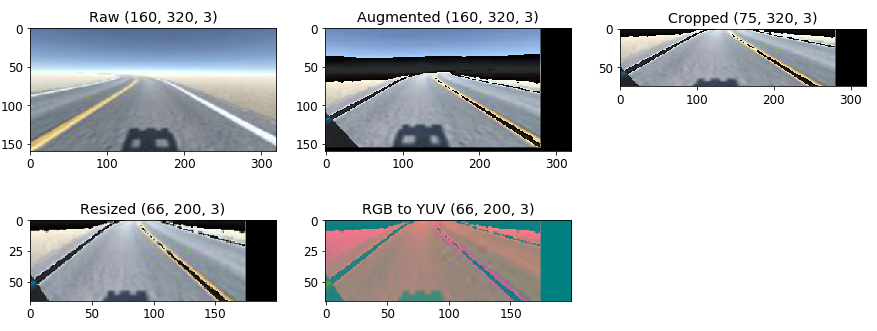
\includegraphics[width=\textwidth]{Figures/AugmentationPreProcessing.png}
 \caption{Stages of image augmentation and pre-processing with array dimensions on each step}
 \label{fig:augpreproc}
\end{figure}

Prior to presenting pixel colour channel values to the network, a number of pre-processing steps have become standard with neural network classifiers and regressors applied to computer vision.

The data distribution depends on the track. Figure \ref{fig:GeneratedTrackPlusHist} shows a normalized histogram of 45410 steering angles obtained in 10 recorded sessions (data directory dataset/unity/smallLoop) corresponding to steering angles. The simulator records at a, computational resources allowing, maximum rate of 60 fps (frames per second). The observed average on the track was approximately 24 fps, representing in this case 31m32s  in approximately 19 laps. The 24 fps average was obtained by recording ("Auto Drive w Rec" option) for one lap, taking approximately 1m41s seconds and generating 2455 frames. The simulator registered fps rates higher than average on straight sections and lower than average on curved sections. This is assumed to be due to computational overheads imposed on the physics engine in the curved sections, resulting in less frames being recorded. The maximum steering angle, is set in the simulator with respect to a car. In this case it is plus or minutes 25 degrees. The normalized value, in the range of -1 to 1 is recorded. Values displayed in the histogram are multiplied by the maximum steering angle. The data shows a high bias towards right turns because the simulated vehicle drives clockwise around the track.
\begin{figure}[ht]
 \centering 
 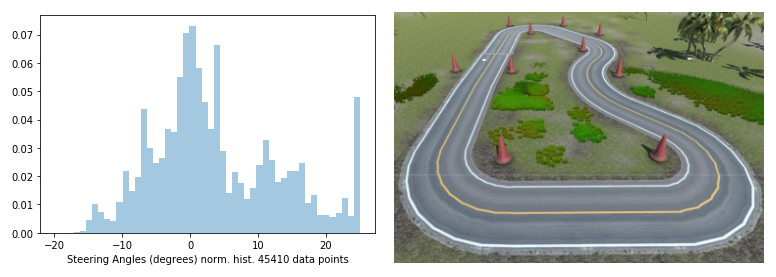
\includegraphics[width=\textwidth]{Figures/GeneratedTrackPlusHistogram.png}
 \caption{Normalized histogram of Unity 3D SDSandbox steering angles for 45410 image frames. The corresponding track (small\_looping\_couse) is shown on the right}
 \label{fig:GeneratedTrackPlusHist}
\end{figure}

Another simulated circuit used was the \textit{Generated Road}, which creates a random path on every run. This can be seen in figure \ref{fig:GeneratedRoadPlusHist}. The total number of frames collected for 15 \textit{Auto Drive w Rec} sessions (saved in dataset/unity/genRoad) was 280727, approximately 3h14m37s. The outliers, mainly to left of histogram, are due to the simulated vehicle being left unattended, reaching the end of the road and continuing into a section with no road markings, becoming stuck in a hard-left turn, until the simulation was switched off and recording halted. The mean and standard deviation, for angles in the range -20 to + 20, are -0.18 and 5.37 degrees respectively. The number of outliers removed was 2204 (0.79\%). It can be seen that when more data points are collected, the bell-shaped curve becomes smoother.

\begin{figure}[ht]
 \centering 
 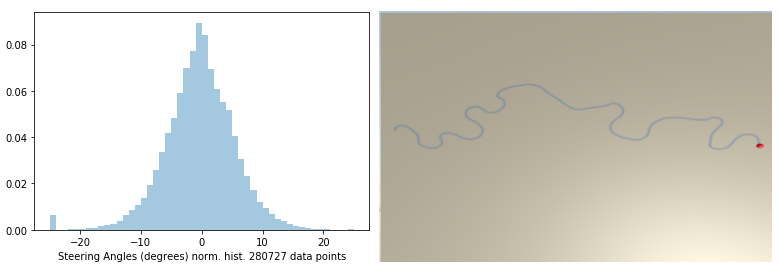
\includegraphics[width=\textwidth]{Figures/GeneratedRoadPlusHistogram.png}
 \caption{Normalized histogram of Unity 3D SDSandbox generated road, steering angles for 280727 image frames. A sample randomly generated road is shown on the right}
 \label{fig:GeneratedRoadPlusHist}
\end{figure}

%\section{Data Augmentation}
%To avoid overfitting, the data is augmented by: cropping the %image to a height band that excluded horizon and car shadow, %resized to required model input size, converted from RGB to YUV, 
% get images from http://localhost:8890/notebooks/augument.ipynb

% \section{Training a model}

\section{Predicting steering angles for a simulated track}

To generated predictions \textit{on-the-fly}, the simulator is run in \textit{Auto Drive w Rec} mode. Once activated, the sends frames over the network using the OpenAI Gym (\cite{brockman2016openai} (TODO FURTHER DISCUSS PLATFORM) framework which sends packets over the network. The packets are sent from simulator using TCP (\cite{rfc793}), include packets \textbf{DESCRIBE PACKETS}.  
\textbf{DESCRIBE HANDSHAKING} \textbf{DESCRIBE TCP} 
\textbf{DESCRIBE GRAPH}
Figure \ref{fig:PredSteeringAnglestcpflowNvidia1} shows a plot of predicted and simulator steering angles. The prediction is for a single image frame sent over the network. As the simulation begins, frames are sent over the network and in this case, captured with tcpflow (\cite{garfinkel2013passive}. A log file was produced. The log file was processed (\cite{JUPYTERNOTEBOOKINAPPENDIX} and created plot. This was for one lap of the \textit{Generated Track}, similar to the track shown in Figure \ref{reffigure}. The actual processing frame rate is approximately 11fps. The y axis is flipped so the plot relates to the path taken by simulated vehicle, the first drop indicating the first right turn, the rise and sharp drop indicating the sharp right turn at the opposite end of the starting line.

\begin{figure}[ht]
 \centering 
 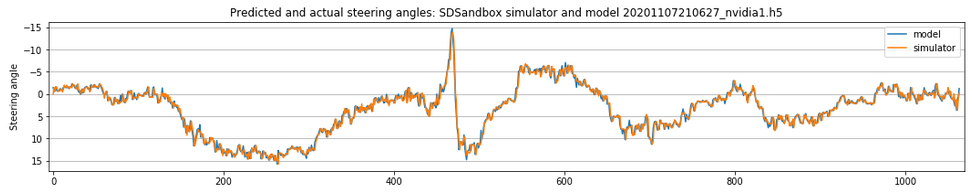
\includegraphics[width=\textwidth]{Figures/PredSteeringAnglestcpflowNvidia1.png}
 \caption{Predicted (blue) and ground-truth simulator (orange) steering angles. The simulator steering angle values in this case are obtained from data packets sent over the TCP network.}
 \label{fig:PredSteeringAnglestcpflowNvidia1}
\end{figure}

Taking this technique one step further, a video can be created using the image sent by simulator, next to the processed image presented to network. Together with the steering angle that would be used by simulator with the steering angle produced by prediction engine (predict\_client.py) which is used by the simulator.
This also can produced a metric representing \textit{goodness-of-steer}, as seen in equation     \ref{eq:goodness_of_steer}:

\begin{equation}
    \label{eq:goodness_of_steer}
    g_s(p,g) = \frac{\sum_i^N \lvert p(i)-g(i) \rvert }{N} \times n_c
\end{equation}
where $p,g$ are prediction and ground truth arrays,  $N$ is the number of predictions and $n_c$ is the normalization constant (25 in example shown, 1 for values not normalized). The sum of the absolute value of the difference between prediction and ground truth values, divided by the number of predictions multiplied by a normalization constant, is the steering error average over all predictions. This error metric is used to compare models quantitatively. For example, in Figure \ref{fig:PredSteeringAnglestcpflowNvidia1} $g_s = 0.59^{\circ}$, that is, on average the model steering is $0.59^{\circ}$ off the ground truth steering on every predicted image frame. 

\section{Identifying rainy images with Amazon Mechanical Turk}

Amazon Mechanical Turk \cite{crowston2012amazon} is an online marketplace where jobs can be outsourced using the \textit{crowsourcing} model  (\cite{vukovic2009crowdsourcing}) which delivers a scalable workforce that may be adjusted in size as required. Mechanical Turk has been referred to as \textit{artificial artificial intelligence} (\cite{dai2011artificial}) where a task requiring human intelligence level, such as labelling an image, can be assigned to a real person, in lieu of writing  a computer algorithm capable of doing so. Mechanical Turk, launched in 2005, was instrumental in labelling the Imagenet (\cite{deng2009imagenet}) dataset which lead to advances in computer vision image recognition with a number of deep (TODO explain "deep" at some point) network architectures ( \cite{krizhevsky2012imagenet}, \cite{he2015deep}, \cite{szegedy2014going} and \cite{simonyan2015deep}). 

For this study Amazon SageMaker Ground Truth (\cite{SageMakerGroundTruthDocumentation2020}) was used. It is a wrapper for Mechanical Turk, and facilitates the process of setting up the image labelling job, especially the UI (user interface) that the labeler workforce must used.  
The aim here is to find segments of real life footage that may contain rain. The Ford AV (\cite{agarwal2020ford}) has sections labeled as "cloudy" so may contain rain. 100 images, chosen at regular intervals, the expectation being this may help narrow down the location of rainy images, if any. To test the accuracy of the service, 5 images with rain are added to the dataset. The expectation being labels for these 5 images will be "rain". 
% https://us-east-2.console.aws.amazon.com/sagemaker/groundtruth?region=us-east-2#/labeling-jobs/create
The unlabelled dataset is stored on AWS S3 (\cite{AmazonS3Documentation2020}). An "Image Classification (Single Label)" "Task type" is chosen, i.e. workers will verify if the proposed label "Rainy image" is correct. The process workflow is shown of Figure \ref{fig:amazon-ground-truth}.

\begin{figure}[ht]
 \centering 
 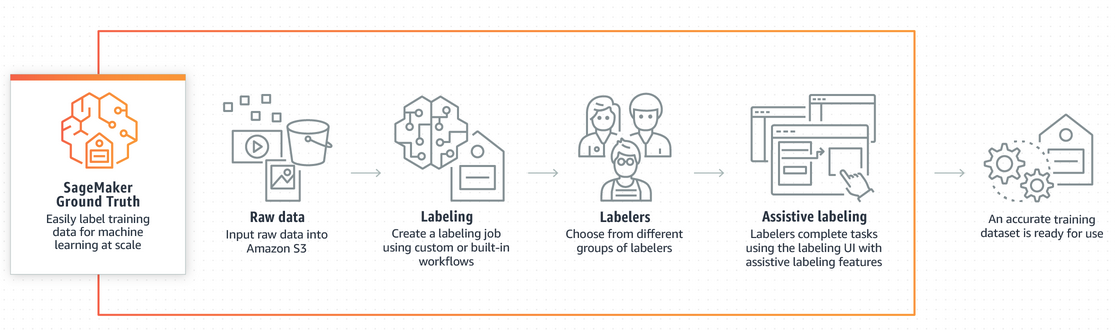
\includegraphics[width=\textwidth]{Figures/SageMakerGroundTruth.png}
 \caption{Amazon SageMaker Ground Truth workflow: a dataset is placed on Amazon S3, labeling job is created, workers label data using a labeling user interface resulting in a labeled dataset}
 \label{fig:amazon-ground-truth}
\end{figure}



\section{Adding rain to images}
% Missing an introduction discussing why this is being done
The synthetic datasets used contain no rain. To test models with rainy images, rain must be added. 
To add rain to the testing images, \textit{Automold Road Augmentation Library} (\cite{Saxena2017}) is used, consisting of a Python module capable of adding rain-like effect to images. Figure \ref{fig:AutomoldRoadAugmentationLibrary} shows on the top row, a real-life image and on the bottom row, an image created by SDSandbox simulator. The columns from left to right have: no rain added, light rain added, heavy rain with a -10 degree slant added and torrential rain with a 20 degree slant added.  
During inference (running steering predictions) the image is (in addition to same pre-processing, and excluding augmentation, performed during training time) processed such that it will contain rain never seen before by the network. The outcome is uncertain, given the effect of random noise on CNNs (see section TODO add section with discussion on one pixel attacks), although the flattening effect of the RGB to YUV transformation (see section TODO add section with RGB to YUV discussion) may have a desirable filtering effect.

\begin{figure}[h!]
\centering
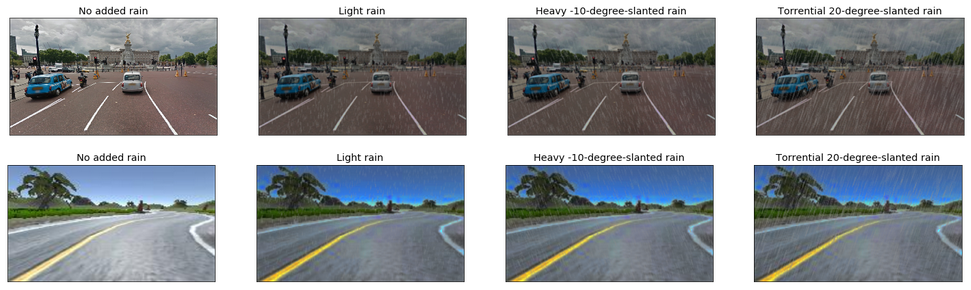
\includegraphics[width=\textwidth]{Figures/AutomoldRain.png}
\caption{Left to right: images}
\label{fig:AutomoldRoadAugmentationLibrary}
\end{figure}

\section{Development environments}

Three development environments are planned to be used, a local environment to run the Unity3D SDSdanbox application, and two additional environments, the Intel Dev-Cloud (\cite{IntelDevCloud2020}) and City University's Camber server (\cite{Camber2019}).
% Further develop running jobs in these environments

\subsection{Digital Images}
Digital images are stored as a square multidimensional matrix. A 100x100 colour images (with values from Red, Green and Blue) is represented as a matrix of dimensions $n x m x c$, where n is the width, m is the height and c is the depth (number of colour channels of the image. Black and white images have c = 1, where the pixel value is either on or off (TBC). Greyscale images also have one channel.

Maybe cite goodfellow once and do a joblot on items.  

Our NVIDIA architecture is very similar to the one proposed by Bojarski et al. 2016. Our alternative AlexNet, GoogleLeNet, VGGNet and ResNet however have much fewer parameters. This is due to the "degradation" problem, where the number of parameters is too large for the dataset, and the network fails to converge.

\section{Datasets}
% What datasets we used and what data was gathered
3 datasets where used. Udacity self-driving real life data, Unity 3D game engine data, and the same datasets with added rain. Figure X shows details of the data.

The datasets are downloaded via script (\cite{Sikar2020}) and structured according to environment (local, Camber or DevCloud).

Two data augmentation libraries were used: \cite{Naoki2016} to add random shifts, flips, crop and change images to YUV format (as per \cite{bojarski2016end} data augmentation method used in the baseline architecture) and \cite{Saxena2017} to add rain and reflections to the testing datasets.

\section{Training and Testing}

The Keras (\cite{chollet2015keras}) deep learning API (Application Programming Interface) written in Python (\cite{van1995python}) and in this case acting as a wrapper around the machine learning library Tensorflow (\cite{abadi2016tensorflow})  was used to create, train and test models.

\subsection{Ford AV Dataset}
% Get details from https://avdata.ford.com/downloads/default.aspx
The Ford Autonomous Vehicle is a 
% angle from IMU
From % https://s23.q4cdn.com/258866874/files/doc_downloads/2020/03/2003.07969.pdf
 (\cite{Applanix}) is a professional-grade, compact,fully  integrated,  turnkey  position  and  orientation  system combining a differential GPS, an inertial measurement unit(IMU)  rated  with  1$^{\circ}$ of  drift  per  hour,  and  a  1024-count wheel encoder to measure the relative position, orientation,velocity,  angular  rate  and  acceleration  estimates  of  the vehicle. The Ford AV data set provides the 6-DOF pose (6DOF pose estimation of objects is the task of estimating the coordinates (X, Y,Z) and rotation angles (Yaw, Pitch and Roll) of an object with respect to a previously established reference coordinate system. (\cite{7005077} ) estimates obtained by integrating the (linear) acceleration and (angular) velocity.
% Note, Ford av authors discussion https://s23.q4cdn.com/258866874/files/doc_downloads/2020/03/2003.07969.pdf
% IEEE on 6DOF estimation from IMU discussion https://ieeexplore.ieee.org/document/7005077

% on converting GPS and IMU measurements to steering angles, see
% http://www.robesafe.uah.es/personal/roberto.arroyo/docs/Almazan13iv.pdf
% We might use a similar technique, time allowing

\subsection{Kitti}

The Kitti dataset TODO add provenance, add description
Data format, steering angle description obtained from oxts/dataformat.txt 
% cat 2011_09_26/2011_09_26_drive_0001_sync/oxts/dataformat.txt
\begin{verbatim}
yaw:   heading (rad),       0 = east,  positive = counter clockwise,\
    range: -pi   .. +pi
\end{verbatim}
Note, this may not be the steering angle - TBC. So additional work may be needed to obtain.
There are some pointers online, a simple approach seems to be:
% https://physics.stackexchange.com/questions/112301/calculating-the-rate-at-which-a-car-turns
This is also an interesting approach:
% http://docs.ros.org/en/kinetic/api/teb_local_planner_tutorials/html/cmd__vel__to__ackermann__drive_8py_source.html
With python code:
\begin{verbatim}
def convert_trans_rot_vel_to_steering_angle(v, omega, wheelbase):
  if omega == 0 or v == 0:
     return 0
  radius = v / omega
  return math.atan(wheelbase / radius)    
\end{verbatim}
Another possible method "Estimation of the Steering Angle Based on Extended Kalman-Filter"  
% http://gvpress.com/journals/IJMUE/vol11_no12/27.pdf
% equations 10 and 11

\subsection{Data balancing}

Class imbalance (\cite{batista2004study}) has an effect on model's accuracy. A heavily outnumbered class may be difficult to learn. Rare events lead to the creation of imbalanced learning scenarios (\cite{krawczyk2016learning}). In the case of self-driving car data, the expectation is that most of steering angles are expected to be close to zero (car driving straight). So some form of undersampling may need to be used to address the issue.






\subsection{Data Augmentation}
The data was augmented with several methods

Describe was additional transformations was performed to enlarge dataset - maybe a discussion that more data is good? With references.


Found this article:
% https://lmb.informatik.uni-freiburg.de/Publications/2015/FDB15/image_orientation.pdf
Would some good suggestions:  
Augmentation. To prevent overfitting, we perform image augmentation, i.e., we
apply random transformations to input samples during network training on the
fly. We use translations (up to 5\% of the image width), brightness adjustment
% in the range [−0.2, 0.2], gamma adjustment with \\gamma \\memberof [−0.5, 0.1] and Gaussian
pixel noise with a standard deviation in the range [0, 0.02].
  
\section{Deep Convolutional Neural Network Models}

In this section all network architectures used are described.

\section{NVIDIA \textit{End to End Learning for Self-Driving Cars} Network Architecture}

The NVIDIA network (\ref{NVIDIA_baseline}) is the baseline sefl-driving architecture used in this study. This comprises three (RGB channel) x 66 (height) x 200 (width) size input layer corresponding to an image presented to network. The input layer is followed by: a normalization layer generating a 3 channel 66 x 200 layer, a 24 5x5 kernel convolutional layer generating 31x98 feature maps, a 36 5x5 kernel convolutional layer generating 14x47 feature maps, a 48 5x5 kernel convolutional layer generating 5x22 size feature maps, a 64 3x3 kernel convolutional layer generating 3x20 size feature maps, a 64 3x3 kernel generating 1x18 size feature maps, a 1164 neuron flattened layer fully connected to a 100 neuron layer, fully connected to a 50 neuron layer, fully connected to a 10 neuron layer, fully connected to a one neuron output layer.  
The first 3 convolutional layers have stride equal 2 and the last 2 convolutional layers have stride equal 1. Padding is equal to zero, resulting in smaller feature maps with every convolutional layer.
The size of feature maps generated by each convolutional layer is determined with equation \ref{eq:feature_map} as described in \cite{dumoulin2018guide}:
\begin{equation}
    \label{eq:feature_map}
    n_{out}= \Big\lfloor\frac{n_{in} + 2p -k}{s} \Big\rfloor +1
\end{equation}
where $n_{out}$ is output size of convolved feature map, $n_{in}$ is input size of image or feature map, $p$, $k$ and $s$ are padding, kernel and stride size respectively.  
 
For example, to determine size of feature maps in the first convolutional layer $n_{out}=\lfloor(66+(2\times0)-5)/2\rfloor)+1=31$, $n_{out}=\lfloor(200+(2\times0)-5)/2\rfloor+1=98$. The Keras (\cite{chollet2015keras}) machine learning framework is used to build the model. The calculation for number of trainable parameters (weights) in a convolutional layer is given in equation \ref{eq:trainable_params}:
\begin{equation}
    \label{eq:trainable_params}
    n_p= m \times n \times  d \times k + d
\end{equation}
where $m$ and $n$ are the convolutional kernel dimensions, $d$ is the number of feature maps in the current layer and $k$ is the number of feature maps in the previous layer. Note $d$ is added to acccount for \textit{bias} term. For example, the number of trainable parameters for the first convolutional layer in \ref{NVIDIA_baseline} is given by $n_p = 5 \times 5 \times 24 \times 3 + 24 = 1,824$. The number of trainable parameters in a fully connected layer is given by equation \ref{eq:trainable-parmas}:
\begin{equation}
    \label{eq:trainable-parmas}
    n_p= m \times n + n
\end{equation}
where $m$ is the number of inputs in previous layer and $n$ is number of neurons in current layer. Note second term $n$ is added to account for \textit{bias} term. For example, for the first fully connected layer in \ref{NVIDIA_baseline} the number of parameters is given by $n_p = 1164 \times 100 = 1,342,092$, where the inputs are values from previous flattened layer, that is, a vectorized representation of the last convolutional layer feature maps.  
The total number of trainable parameters generated by Keras is 1,595,511. This does not agree with the total given by \cite{bojarski2016end}, who state their "network  has  about (...) 250 thousand parameters". Total memory required to store parameters assuming 32-bit float data type, is 6MB given by $1,595,511 \times 4 \div 1,024 \div 1,024$.

Since the NVIDIA model is based on work by \cite{krizhevsky2012imagenet}, "dropout" (\cite{hinton2012improving}) is assumed to have been used, with 50\% dropout probability on every layer.  
Dropout removes neurons randomly and helps prevent overfitting, where a model performs well on training data and poorly on testing data, by preventing co-adaptation, resulting in neurons that can detect useful features in the multitude of contexts it must operate, and help the network produce the correct answer.
As per correspondence with co-author(\ref{corr_with_authors} additional training hyperparameters are MSE (loss function) 
adadelta (optimizer), "learning rate: 1e-4 (but not really used in adadelta)" and 0.25 dropout.
Additional assumptions on training include: 128 example batch size, weights initialized from a zero-mean normal distribution with standard deviation 0.01 and biases mostly initialized to 1 as per \cite{krizhevsky2012imagenet}, which applied to this baseline architecture initializes all biases to 1, except in convolutional layers 1 and 5, where biases are initialized to 0. Details in source code src/models.py, nivia\_baseline function.  


% TODO need to incorporate section 5    Details of learning of Krizhesvky et al i.e.
%We trained our models using stochastic gradient descent with a batch size of 128 examples, momentum of 0.9, andw eight decay of 0.0005. ETC

% Since the weights are not initialized properly and groups of neurons end up in the same local minima, according to their (similar) initialization.
% To overcome this, you could use dropout / drop connect to break symmetry.
% https://stats.stackexchange.com/questions/181264/how-does-co-adaptation-occur-in-deep-neural-nets

% NB no reference to "Alexnet" in original or NVIDIA articles - clean up required.
%For example, in the classic Alexnet (\cite{krizhevsky2012imagenet}) architecture, with input %image size 224x224, kernel size 11, padding equal zero and stride = 4, the resulting feature %map size in the first convolutional layer is 55x55. 
%Alexnet has an input layer with dimensions 224x224x3, where 3 is the number of channels (RGB %image), the second layer has dimensions 55x55x48, the third convolutional layer has %dimensions 27x27x128 and so on. This is typical of deep network architectures, decreasing %feature map sizes with increasing number of channels as network depth increases.
`  

\textbf{Discussion on the number of parameters required given size of dataset.}  
We also need a discussion on deep regression models as suggested by \cite{lathuilire2018comprehensive}. This is the main difference between the NVIDIA and additional models, the NVIDIA model is a regression model while the models we compare and contrast with NVIDIA are classification models built specifically for the ILSVC  competitiion.

\subsection{ResNet}

Discuss the concept of "residuals". ResNet makes use of skip-connections (spelling), these "network architecture
designs (e.g., skip connections) produce loss functions that train easier", producing smoother loss surfaces (\cite{li2017visualizing})  
The "Degradation problem itself stems from the fact that it is easier to learn 0 than to learn 1"   https://www.youtube.com/watch?v=jio04YvgraU
"if an identity mapping were optimal, it would be easier to push the residual to zero than to fit an identity mapping by a stack of nonlinear layers" \cite{he2015deep}.  
Explain what variation A, B or C we will be using (zero padding, weights * x, etc.  
"Essemble" of ResNets was used.  
18 layers seems to be a threshold, beyond that, training becomes difficult. Skip connections make deeper networks, i.e. networks with more layers, easier to train compared to networks without skip connections.  
Another wording, deeper neural networks (i.e. layer count equal or greater than 20) become increasingly difficult to train, generating poorer accuracy than deep networks with less than 20 layers. This is known as "degradation problem" (citation needed). Skip connections make deeper architectures easier to train, by smoothing the loss function.

\subsection{GoogleLeNet}

This network (\cite{szegedy2014going}) was the winning entry in the ILSVCC 2014 Classification Challenge. It uses the LeNet-5 (\cite{Lecun98gradient-basedlearning}) model as a starting point, following the now traditional design of ConvNets with the addition of \textit{Inception} modules as introduced by \cite{lin2013network} in the \textit{Network in Network} model.

\begin{figure}[ht]
 \centering 
 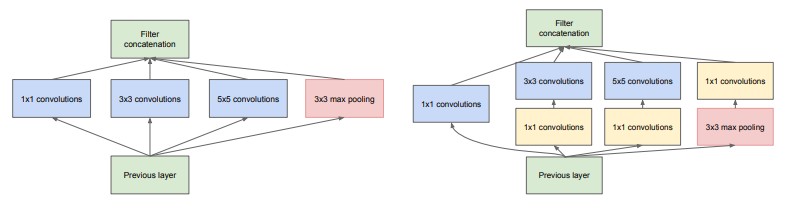
\includegraphics[width=\columnwidth]{Figures/InceptionModules.png}
 \caption{Inception naive (left) and dimension reduction model (right)}
 \label{fig:inception_modules}
\end{figure}

The designers of the GoogleLeNet architecture state that power and memory use is important to consider and aim to keep a computation budget of 1.5 billion multiply adds at inference time such that the resulting model could be used in practice at a reasonable cost.

The architecture contains 22 layers where all

\subsection{Deep Regression Models}
Explain the process of transforming these models (except NVIDIA) into regression models, maybe cite \cite{lathuilire2018comprehensive} or papers cited therein.

Paper is referred to by this discussion: 
% https://stats.stackexchange.com/questions/335836/cnn-architectures-for-regression
A somewhat more succinct definition of the procedure:  
% https://stats.stackexchange.com/questions/456126/could-resnet-curve-be-used-for-a-regression-problem-e-g-housing-price-predicti
Just to make it clear, a regression problem is one whose target is continuous and not discrete. In this sense you can make any Neural Network that is primarily used for classification a regressor, with minimal changes. Namely it needs to end with 1 neuron, no activation function and a proper loss function (e.g. mean squared error). For example, object detection is in its core a regression problem because you are trying to predict coordinates. Any ResNet could be used for these problems

\subsection{Binning/Quantization}
Describe this approach, if we get that far, to use an alternative to regression models, whereby we may bin the outputs. This could potentially simplify the model. Also, depending on track, we could have narrower bins around zero degrees, i.e. finer control and wider bins away from zero degrees, i.e. coarser control. Or vice-versa - experimentation required.

\subsection{Training}

We might want to add that training was done on AWS GPUs following   
https://aws.amazon.com/blogs/machine-learning/train-deep-learning-models-on-gpus-using-amazon-ec2-spot-instances/  


\section{Evalutation}
This section discussed the evaluation benchmarks, here we discuss the evaluation environment (Unity 3D game engine) and how it was used to both generate data and evaluate the models.

%% Udacity
%% see https://arxiv.org/pdf/1912.05440.pdf
%% for discussion on using rmse as error metric


